\documentclass{scrartcl}

\usepackage{unicode-math}

\usepackage{tikz}
\usetikzlibrary{babel,cd,hobby,shapes.misc,3d}
\tikzcdset{arrow style=math font}
 
\tikzset{cross/.style={cross out, draw, solid, thin, 
         minimum size=2*(#1-\pgflinewidth), 
         inner sep=0pt, outer sep=0pt},
         cross/.default={3}}

\begin{document}


\begin{tikzcd}[ampersand replacement=\&]
  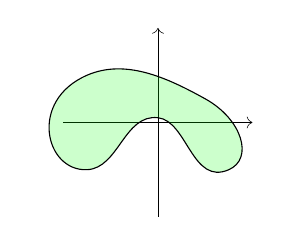
\begin{tikzpicture}[use Hobby shortcut,scale=0.3,baseline=0]
  \draw[->, very thin] (-4,0) -- (4,0);
  \draw[->, very thin] (0,-4) -- (0,4);

  \filldraw [fill opacity=0.2,fill=green] ([closed]2,1) .. (-3,2) .. (-3,-2) .. (0,0.2) .. (3,-2);
\end{tikzpicture} \arrow[r] \&%
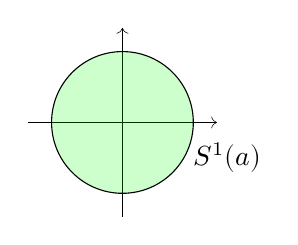
\begin{tikzpicture}[scale=0.3,baseline=0]
  \draw[->, very thin] (-4,0) -- (4,0);
  \draw[->, very thin] (0,-4) -- (0,4);

  \filldraw[fill opacity=0.2,fill=green] (0,0) circle [radius=3];
  \draw (0,0) (-30:3) node[anchor=west]{$S^1(a)$};
\end{tikzpicture}
\end{tikzcd}

% Auroux system
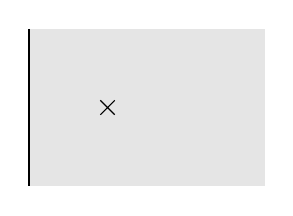
\begin{tikzpicture}
  \fill[opacity=0.1] (0,1) rectangle (3,-1);
  \draw[thick] (0,1) -- (0,-1) (1,0) node[cross] {};
\end{tikzpicture}

% Auroux fibration
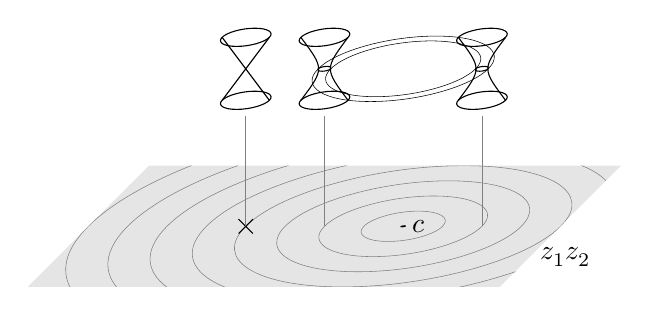
\begin{tikzpicture}[scale=2]
  \begin{scope}[canvas is xz plane at y=0]
    \draw (2,.5) node[anchor=west] {$z_1 z_2$};
    \clip (-1,-1) rectangle (2,1);
    \fill[opacity=0.1] (-1,-1) rectangle (2,1);
    \foreach \x in {0.25,0.5,...,2.0}
      \draw[very thin, gray] (1,0) circle [radius=\x];
    \fill (0,0) node[cross] {} (1,0) circle [radius=.5pt] node[anchor=west] {$c$};
  \end{scope}
  \foreach \x in {0.8,1.2} {
    \begin{scope}[canvas is xz plane at y=\x]
      \draw (0,0) circle[radius=0.15] (0.5,0) circle[radius=0.15] (1.5,0) circle[radius=0.15];
    \end{scope}
  }
  \begin{scope}[canvas is xz plane at y=1.0]
    \foreach \x in {0.5,1.5}
      \draw (\x,0) circle [radius=0.04];
    \draw[very thin] (1,0) circle [radius=0.5-0.04] circle [radius=0.5+.04];
  \end{scope}
  \begin{scope}[canvas is xy plane at z=0]
    \draw (.15,0.8) -- (-.15,1.2) (.15,1.2) -- (-.15,0.8);
    \foreach \x in {0.5,1.5}
      \draw (\x-.15,0.8) .. controls (\x,1.0) .. (\x-.15,1.2) (\x+.15,1.2) .. controls (\x,1.0) .. (\x+.15,0.8);
    \foreach \x in {0,0.5,1.5}
      \draw[very thin,gray] (\x,0) -- (\x,0.7);
  \end{scope}
\end{tikzpicture}

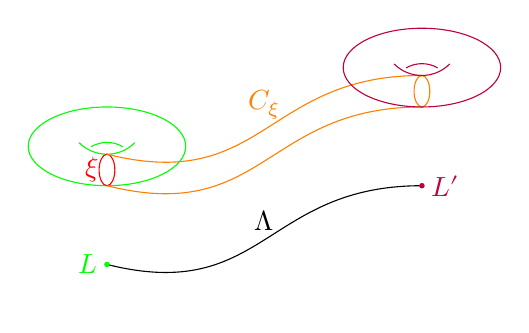
\begin{tikzpicture}
  \draw (-2,-0.5) .. controls ++(2,-0.5) and ++(-2,0) .. node[anchor=south] {$Λ$} (2,0.5);
  \fill[green] (-2,-.5) circle [radius=1pt] node [anchor=east] {$L$};
  \fill[purple] (2,.5) circle [radius=1pt] node[anchor=west] {$L'$};

  \draw[green] (-2,1) circle [x radius=1,y radius=0.5]
    (-2,1.4) +(-135:0.5) arc [start angle=-135,end angle=-45,radius=0.5]
    (-2,0.65) +(60:0.4) arc [start angle=60,end angle=120,radius=0.4];
  \draw[red] (-2,0.7) circle [x radius=0.1,y radius=0.2] node[anchor=east] {$ξ$};

  \draw[orange] (-2,0.9) .. controls ++(2,-0.5) and ++(-2,0) .. node[anchor=south] {$C_ξ$} (2,1.9)
  (-2,0.5) .. controls ++(2,-0.5) and ++(-2,0) .. (2,1.5);
  \draw[orange] (2,1.7) circle [x radius=0.1,y radius=0.2];

  \draw[purple] (2,2) circle [x radius=1,y radius=0.5]
    (2,2.4) +(-135:0.5) arc [start angle=-135,end angle=-45,radius=0.5]
    (2,1.65) +(60:0.4) arc [start angle=60,end angle=120,radius=0.4];
\end{tikzpicture}


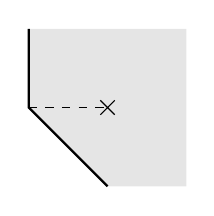
\begin{tikzpicture}
  \fill[opacity=0.1] (0,1) -- (0,0) -- (1,-1) -- (2,-1) -- (2,1);
  \draw[thick] (0,1) -- (0,0) -- (1,-1);
  \draw[dashed] (0,0) -- (1,0) node[cross] {};
\end{tikzpicture}


% Nodal Slide
\begin{tikzcd}
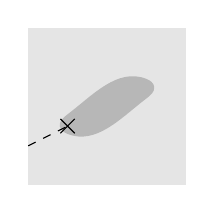
\begin{tikzpicture}[scale=0.5,use Hobby shortcut]
  \fill[opacity=0.1] (0,2) rectangle (4,-2);
  \fill[opacity=0.2] ([closed]1,-.2) .. (0.8,-.5) .. (1,-.7) .. (3,0.2) .. (3.2,0.5) .. (3,0.7);
  \draw[dashed] (0,-1) -- (1,-0.5) node[cross] {};

\end{tikzpicture} \arrow[r] &%
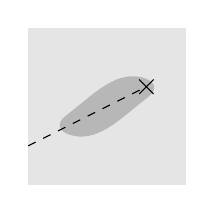
\begin{tikzpicture}[scale=0.5,use Hobby shortcut]
  \fill[opacity=0.1] (0,2) rectangle (4,-2);
  \fill[opacity=0.2] ([closed]1,-.2) .. (0.8,-.5) .. (1,-.7) .. (3,0.2) .. (3.2,0.5) .. (3,0.7);
  \draw[dashed] (0,-1) -- (3,0.5) node[cross] {};
\end{tikzpicture}
\end{tikzcd}

% Nodal trade
\begin{tikzcd}

\begin{tikzpicture}[use Hobby shortcut]
  \draw[thick] (0,2) -- (0,0) -- (2,0);
  \clip (0,2) rectangle (2,0);
  \fill[opacity=0.1] (0,2) rectangle (2,0);

  \fill[opacity=0.2] ([closed]0,0.2) .. (1.1,1.2) .. (1.2,1.1) .. (0.2,0) .. (-.2,-.2);
\end{tikzpicture} \arrow[r,bend left] &%
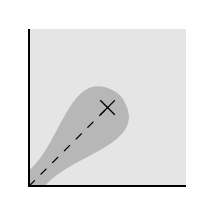
\begin{tikzpicture}[use Hobby shortcut]
  \draw[thick] (0,2) -- (0,0) -- (2,0);
  \clip (0,2) rectangle (2,0);
  \fill[opacity=0.1] (0,2) rectangle (2,0);

  \draw[dashed] (0,0) -- (1,1) node[cross] {};

  \fill[opacity=0.2] ([closed]0,0.2) .. (1.1,1.2) .. (1.2,1.1) .. (0.2,0) .. (-.2,-.2);
\end{tikzpicture}
\end{tikzcd}

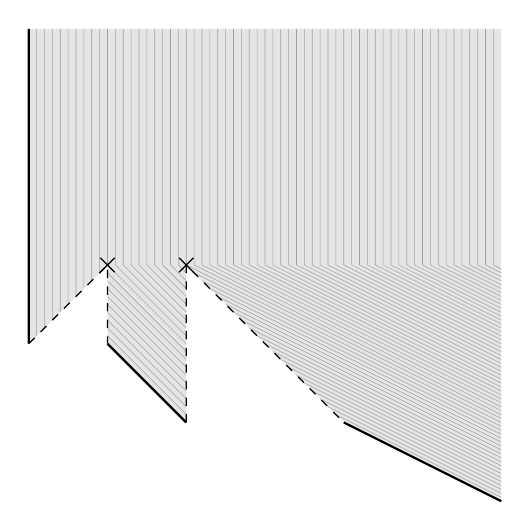
\begin{tikzpicture}
  \fill[opacity=0.1] (0,3) -- (0,-1) -- (1,0) -- (1,-1) -- (2,-2) -- (2,0) -- (4,-2) -- (6,-3) -- (6,3);

  %\draw[opacity=0.3, very thick] (0,0) -- (6,0);
  \foreach \l in {0.1,0.2,...,.9}
    \draw[opacity=0.3, very thin] (\l,3) -- (\l,\l-1)
      (1,\l-1) -- (2,\l-2)
      (4-\l,\l-2) -- (6,\l/2-3);
  \foreach \l in {1.0,1.1,...,2.0}
    \draw[opacity=0.3, very thin] (\l,3) -- (\l,0)
      (\l,0) -- (2,\l-2)
      (4-\l,\l-2) -- (6,\l/2-3);
  \foreach \l in {2.0,2.1,...,6.0}
    \draw[opacity=0.3, very thin] (\l,3) -- (\l,0)
      (\l,0) -- (6,\l/2-3);

    \draw[thick] (0,3) -- (0,-1) (1,-1) -- (2,-2) (4,-2) -- (6,-3);
  \draw[dashed] (0,-1) -- (1,0) node[cross] {} -- (1,-1) (2,-2) -- (2,0) node[cross] {} -- (4,-2) -- (6,-3);
\end{tikzpicture}

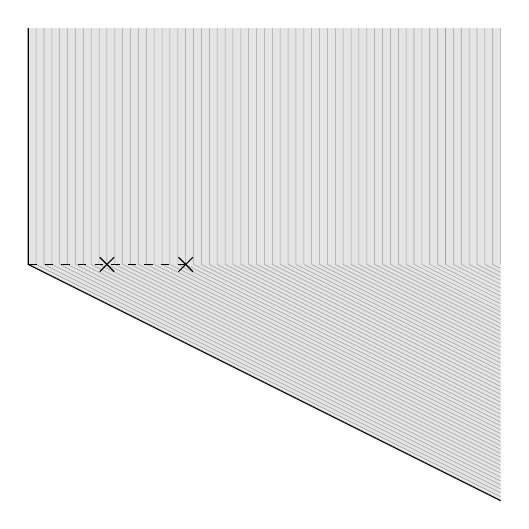
\begin{tikzpicture}
  \fill[opacity=0.1] (0,3) -- (0,0) -- (6,-3) -- (6,3);
  \foreach \l in {0.1,0.2,...,6.0}
    \draw[opacity=0.3, very thin] (\l,3) -- (\l,0)
      (\l,0) -- (6,\l/2-3);
  \draw (0,3) -- (0,0) -- (6,-3);
  \draw[dashed] (0,0) -- (1,0) node[cross] {} -- (2,0) node[cross] {};
\end{tikzpicture}

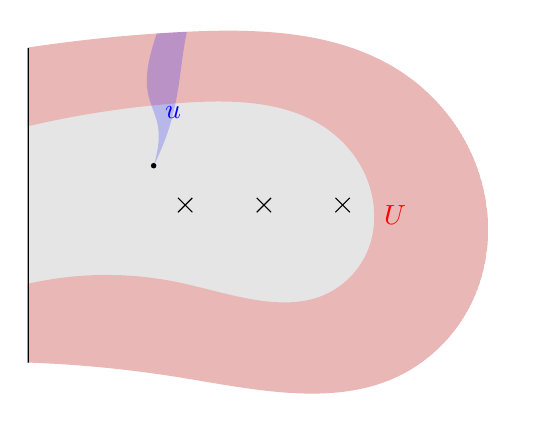
\begin{tikzpicture}[use Hobby shortcut]
  \clip (0,2) -- (0,-2) .. (2,-2.2) .. (5,-2) .. (5,1.5) .. (2,2.2) .. (0,2);
  \fill[opacity=0.1] (0,3) rectangle (6,-3);
  \fill[red,fill opacity=0.2,text opacity=1] (0,2) -- (0,1) .. (2,1.3) .. (4,.8) .. node[anchor=west] {$U$} (4,-1) .. (2,-1) .. (0,-1) --
    (0,-2) .. (2,-2.2) .. (5,-2) .. (5,1.5) .. (2,2.2) .. (0,2);

  \draw[thick] (0,2) -- (0,-2) (2,0) node[cross] {} (3,0) node[cross] {} (4,0) node[cross] {};

  \fill (1.6,0.5) circle (1pt);
  \fill[blue,fill opacity=0.2,text opacity=1] (1.6,0.5) .. controls ++(0.5,1) and ++(-.5,-1) .. node[near start] {$u$} (2.3,3) -- (2,3) .. controls ++(-1,-2) and ++(0.3,1) .. (1.6,0.5);

\end{tikzpicture}

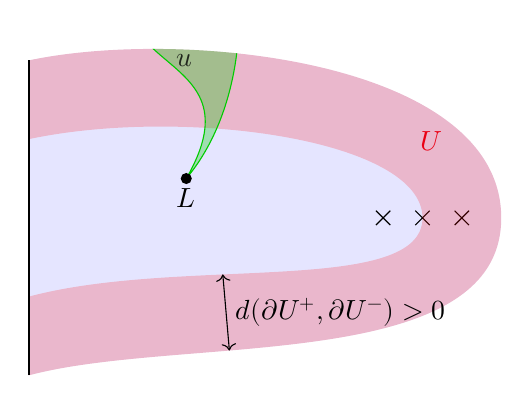
\begin{tikzpicture}
  \coordinate (L) at (2,0.5);
  \begin{scope}
    \clip (0,2) .. controls +(12:2) and +(0,2) .. node[near end,anchor=north east,red] {$U$} (6,0) .. controls +(0,-2) and +(15:2) .. coordinate[pos=0.65] (outer shell) (0,-2);
    \fill[blue,opacity=0.1](0,-3) rectangle (7,3);
    \foreach \x in {4.5,5,5.5}
      \draw (\x,0) node[cross] {};
      \fill[red,opacity=0.2] (0,1) .. controls +(12:2) and +(0,1) .. (5,0) .. controls +(0,-1) and +(15:2) .. coordinate[pos=0.62] (inner shell) (0,-1) -- (0,-3) -- (6,-3) -- (6,3) -- (0,3);
    \filldraw[green!80!black,fill opacity=0.3,text opacity=0.8] (L) .. node[anchor=west,black] {$u$} controls +(60:2) and +(-120:2) .. +(-.5,3) .. controls +(60:2) and +(50:2) .. (L);
    \fill (L) circle[radius=2pt] node[anchor=north] {$L$};
  \end{scope}
  \draw[<->] (outer shell) -- node[anchor=west] {$d(∂U^+,∂U^-) > 0$} (inner shell);
  \draw[thick] (0,-2) -- (0,2);
\end{tikzpicture}

  
\end{document}
